\documentclass[oneside,a4paper,14pt]{extarticle}
\usepackage[a4paper,letterpaper,top=20mm,bottom=20mm,left=20mm,right=10mm]{geometry}
\usepackage[russian]{babel}
\usepackage{indentfirst}
\usepackage{graphicx}
\usepackage{caption}
\usepackage{titlesec}
\usepackage{minted, fancyvrb}
\usepackage{hyperref}
\usepackage{enumitem}

% Форматирование листингов с кодом
\setminted{style = rainbow_dash, fontsize = \small} % https://pygments.org/styles/  

% Форматирование заголовков
\titleformat{\section}{\normalsize\bfseries}{\thesection}{1em}{}
\titleformat{\subsection}{\normalsize\bfseries}{\thesubsection}{1em}{}
\titleformat{\subsubsection}{\normalsize\bfseries}{\thesubsubsection}{1em}{}

% Интерлиньяж и абзац
\renewcommand\baselinestretch{1.33}

\setlength{\parindent}{1.25cm}  % длина красной строки

% Для всех списков
\setlist[enumerate]{
  left=\parindent,       % отступ слева
  label=\arabic*.,       % цифры
  itemsep=0pt,           % расстояние между пунктами
  topsep=5pt,            % отступ сверху
  partopsep=0pt,         % дополнительный отступ сверху, если абзац до списка
  parsep=0pt             % отступ между абзацами внутри пункта
}

\setlist[itemize]{
  left=\parindent,       % отступ слева
  itemsep=0pt,           % расстояние между пунктами
  topsep=5pt,            % отступ сверху
  partopsep=0pt,
  parsep=0pt
}

% Гиперссылки
\hypersetup{
  colorlinks=true,
  linkcolor=black,
  urlcolor=blue,
  pdfborder={0 0 0},
  pdftitle={Пользовательские функции и триггеры в PostgreSQL},
  pdfauthor={Черкасов А.А.}
}

\begin{document}

\newpage
\thispagestyle{empty}
\begin{center}
  МИНИСТЕРСТВО НАУКИ И ВЫСШЕГО ОБРАЗОВАНИЯ РОССИЙСКОЙ ФЕДЕРАЦИИ ФЕДЕРАЛЬНОЕ ГОСУДАРСТВЕННОЕ БЮДЖЕТНОЕ ОБРАЗОВАТЕЛЬНОЕ УЧРЕЖДЕНИЕ ВЫСШЕГО ОБРАЗОВАНИЯ\\
  «ВЯТСКИЙ ГОСУДАРСТВЕННЫЙ УНИВЕРСИТЕТ»\\
  Институт математики и информационных систем\\
  Факультет автоматики и вычислительной техники\\
  Кафедра электронных вычислительных машин
\end{center}
\vspace{10mm}

\hfill
\begin{tabular}{l}
  \footnotesize Дата сдачи на проверку:                                          \\
  \footnotesize <<\rule[-1mm]{5mm}{0.10mm}\/>>\rule[-1mm]{20mm}{0.10mm}\ 2025 г. \\
  \footnotesize Проверено:                                                       \\
  \footnotesize <<\rule[-1mm]{5mm}{0.10mm}\/>>\rule[-1mm]{20mm}{0.10mm}\ 2025 г. \\
\end{tabular}
\vfill

\begin{center}
  Пользовательские функции и триггеры в PostgreSQL.\\
  Отчёт по лабораторной работе №3\\
  по дисциплине\\
  <<Управление данными>>\\
\end{center}
\vspace{25mm}
\noindent
\begin{tabular}{ll}
  Разработал студент гр. ИВТб-2301-05-00 & \hspace{18mm}\rule[-1mm]{30mm}{0.10mm}\,/Черкасов А. А./ \\
                                         & \hspace{25.5mm}\footnotesize(подпись)                    \\
  Старший Преподователь                  & \hspace{18mm}\rule[-1mm]{30mm}{0.10mm}\,/Клюкин В. Л./   \\
                                         & \hspace{25.5mm}\footnotesize(подпись)                    \\
\end{tabular}

\noindent
\begin{tabular}{lp{58mm}r}
  Работа защищена &  & \hspace{13mm}<<\rule[-1mm]{5mm}{0.10mm}\/>>\rule[-1mm]{30mm}{0.10mm}\ 2025 г.
\end{tabular}
\vfill

\begin{center}
  Киров\\
  2025
\end{center}

\newpage\thispagestyle{plain}

\section*{Цели лабораторной работы}
\begin{itemize}
  \item[$-$] познакомиться с созданием пользовательских функций и триггеров в PostgreSQL;
  \item[$-$] освоить работу с составными типами данных и массивами;
  \item[$-$] изучить основы работы с процедурным языком PL/pgSQL.
\end{itemize}

\section*{Задание}
\begin{enumerate}
  \item Для таблицы \texttt{devices} создать функцию \texttt{save\_devices}, выполняющую вставку или обновление записи и возвращающую её \texttt{id}.
  \item Для таблицы \texttt{hubs} (на которую ссылаются другие таблицы) создать функцию \texttt{delete\_hubs}, проверяющую наличие внешних ссылок и выдающую ошибку при их наличии.
  \item Для таблицы \texttt{devices} (содержащей числовой столбец \texttt{id}) создать функцию, возвращающую \texttt{SETOF} строк с \texttt{id} $\geq$ заданного значения.
  \item Создать составной тип \texttt{device\_info} и функцию фильтрации массива объектов этого типа.
  \item Создать таблицу лога \texttt{log\_devices} и триггер для фиксации изменений имени устройства.
  \item Реализовать функцию с динамически формируемым SQL-запросом.
\end{enumerate}

\clearpage
\section*{Тема БД: <<Система управления умным домом>>}
База данных предназначена для хранения информации о пользователях, хабах и устройствах умного дома, а также событий, которые генерируют эти устройства. Она обеспечивает:
\begin{itemize}
  \item[$-$] регистрацию и управление пользователями;
  \item[$-$] хранение информации о хабах и их местоположении;
  \item[$-$] классификацию устройств по типам и отслеживание их состояния;
  \item[$-$] фиксацию событий устройств для мониторинга и анализа.
\end{itemize}

\section*{Реализация функций и триггеров}

Все функции и триггеры реализованы на процедурном языке PL/pgSQL и описаны в файле \texttt{functions\_triggers.sql}.

\subsection*{1. Функция \texttt{save\_devices}}

Функция принимает параметры устройства и выполняет вставку новой записи (если \texttt{\_id IS NULL}) или обновление существующей. Возвращает идентификатор обработанной записи.

\begin{minted}{sql}
  SELECT save_devices(NULL, 1, 4, 'New Smart Socket', '{"power": "off"}');
  SELECT save_devices(1, 1, 1, 'Main Ceiling Lamp', '{"power": "on", "brightness": 80}');
\end{minted}

\begin{figure}[H]
  \centering
  
\includegraphics[width=0.425\textwidth]{pics/save_devices_1.png}
  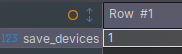
\includegraphics[width=0.425\textwidth]{pics/save_devices_2.png}
  \caption*{Рисунок 1.1 - Вывод функции save\_devices.}
\end{figure}

Проверка:\\
\begin{minted}{sql}
  SELECT id, name, status FROM devices WHERE id IN (1, 7);
\end{minted}

\begin{figure}[H]
  \centering
  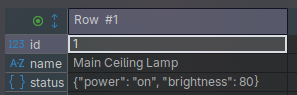
\includegraphics[width=0.5\textwidth]{pics/check.png}
  \caption*{Рисунок 1.2 - Проверка функции save\_devices.}
\end{figure}

\subsection*{2. Функция \texttt{delete\_hubs}}

Перед удалением хаба проверяется наличие связанных устройств. При наличии внешних ссылок генерируется исключение:
\begin{center}
  \texttt{«невозможно выполнить удаление, так как есть внешние ссылки.»}
\end{center}

Для корректной работы ограничение внешнего ключа в таблице \texttt{devices} изменено на \texttt{ON DELETE RESTRICT}.

\begin{minted}{sql}
  -- Попытка удалить хаб с привязанными устройствами (id=1)
SELECT delete_hubs(1);
-- Результат: ОШИБКА: невозможно выполнить удаление, так как есть внешние ссылки.

-- Удаление пустого хаба (если бы он был) — в нашем случае все хабы заняты,
-- но для демонстрации можно временно удалить устройства:
DELETE FROM devices WHERE hub_id = 4;
SELECT delete_hubs(4); -- Успешно
\end{minted}

\begin{figure}[H]
  \centering
  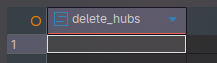
\includegraphics[width=0.5\textwidth]{pics/delete_hubs.png}
  \caption*{Рисунок 2 - Вывод функции delete\_hubs -- Успешно удалён.}
\end{figure}

\subsection*{3. Функция фильтрации \texttt{filter\_devices\_by\_id}}

Возвращает все устройства, у которых \texttt{id} больше или равен заданному значению.

\begin{minted}{sql}
SELECT * FROM filter_devices_by_id(5);
\end{minted}

\begin{figure}[H]
  \centering
  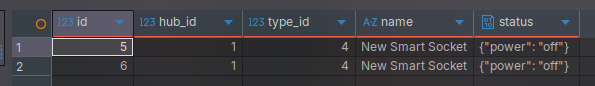
\includegraphics[width=0.95\textwidth]{pics/filter_devices_by_id.png}
  \caption*{Рисунок 3 - Вывод функции filter\_device\_by\_id.}
\end{figure}

\subsection*{4. Составной тип и фильтрация массива}

Создан составной тип:
\begin{minted}{sql}
create type device_info as (
  id bigint,
  name varchar(100),
  type_name varchar(50),
  hub_name varchar(100)
);
\end{minted}

Функция \texttt{filter\_device\_array} принимает массив объектов типа \texttt{device\_info} и возвращает отфильтрованный массив.

\begin{minted}{sql}
SELECT filter_device_array(
    ARRAY(
        SELECT (d.id, d.name, dt.type_name, h.name)::device_info
        FROM devices d
        JOIN device_types dt ON d.type_id = dt.id
        JOIN hubs h ON d.hub_id = h.id
    ),
    5
);
\end{minted}

\begin{figure}[H]
  \centering
  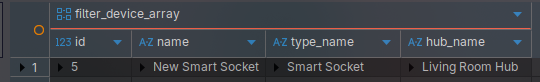
\includegraphics[width=0.95\textwidth]{pics/filter_device_array.png}
  \caption*{Рисунок 4 - Вывод функции filter\_devices\_array.}
\end{figure}

\subsection*{5. Таблица лога и триггер}

Создана таблица \texttt{log\_devices} для фиксации изменений имени устройств. Триггер \texttt{trigger\_log\_devices} срабатывает после операций \texttt{INSERT} и \texttt{UPDATE} и записывает старое и новое значение имени.

\begin{minted}{sql}
-- 5. таблица лога и триггер
create table if not exists log_devices (
  id bigserial primary key,
  device_id bigint references devices(id),
  change_time timestamp default now(),
  old_name varchar(100),
  new_name varchar(100)
);

create or replace function log_device_change()
returns trigger as $$
begin
  if tg_op = 'INSERT' then
    insert into log_devices (device_id, new_name)
    values (NEW.id, NEW.name);
  elsif tg_op = 'UPDATE' then
    insert into log_devices (device_id, old_name, new_name)
    values (NEW.id, OLD.name, NEW.name);
  end if;
  return NEW;
end;
$$ language plpgsql;

drop trigger if exists trigger_log_devices on devices;
create trigger trigger_log_devices
after insert or update on devices
for each row
execute function log_device_change();
\end{minted}

\begin{figure}[H]
  \centering
  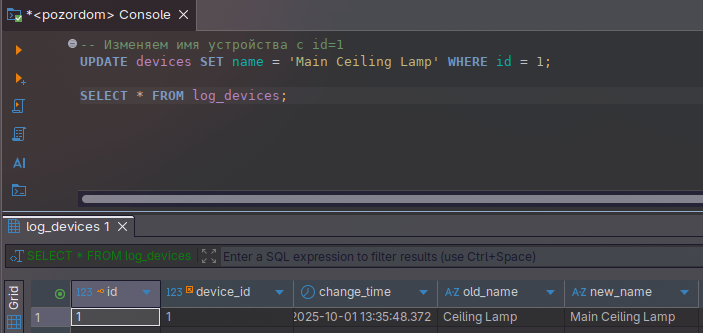
\includegraphics[width=0.95\textwidth]{pics/log_devices.png}
  \caption*{Рисунок 5 - Вывод функции log\_devices.}
\end{figure}

\subsection*{6. Функция с динамическим SQL}

Функция \texttt{get\_column\_value} принимает имя таблицы, имя столбца и идентификатор записи, формирует и выполняет динамический SQL-запрос, возвращая значение указанного столбца.

\begin{minted}{sql}
create or replace function get_column_value(
  table_name text,
  column_name text,
  record_id bigint
)
returns text as $$
declare
  result text;
begin
  execute format(
    'select %I from %I where id = $1',
    column_name, table_name
  )
  into result
  using record_id;
  return result;
end;
\end{minted}

\begin{figure}[H]
  \centering
  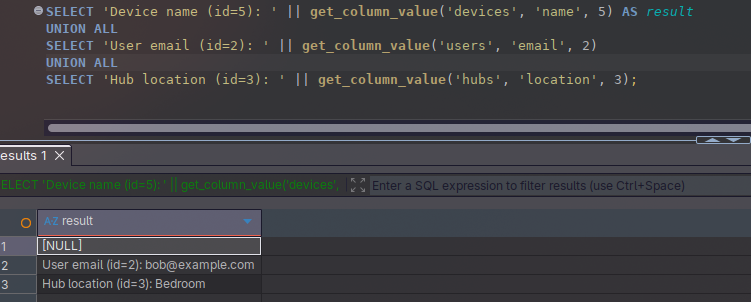
\includegraphics[width=0.95\textwidth]{pics/get_colomn_value.png}
  \caption*{Рисунок 6 - Вывод функции get\_colomn\_value.}
\end{figure}

\section*{Вывод}

В ходе выполнения лабораторной работы №3 были освоены механизмы создания пользовательских функций и триггеров в PostgreSQL. Реализованы функции для безопасной вставки, обновления и удаления записей с проверкой ссылочной целостности. Созданы составной тип и функция для работы с массивами. Реализовано логирование изменений с помощью триггера. Также освоено использование динамических SQL-запросов. Все функции написаны на процедурном языке PL/pgSQL и протестированы на корректность работы.

\newpage

\section*{Приложение А1. Исходный код}
\inputminted{Dockerfile}{../Containerfile}

\section*{Приложение А2. Функции и триггеры}
\inputminted{sql}{code/functions_triggers.sql}

\end{document}